\section{Introduction}

\subsection{Présentation du problème}

Le problème du réveil des robots consiste en un robot éveillé et des robots endormis dans un disque autour de lui. Un robot éveillé peut aller vers d'autres robots pour les réveiller et l'objectif est de réveiller tous les robots le plus vite possible.

\begin{figure}[h!]
  \centering
  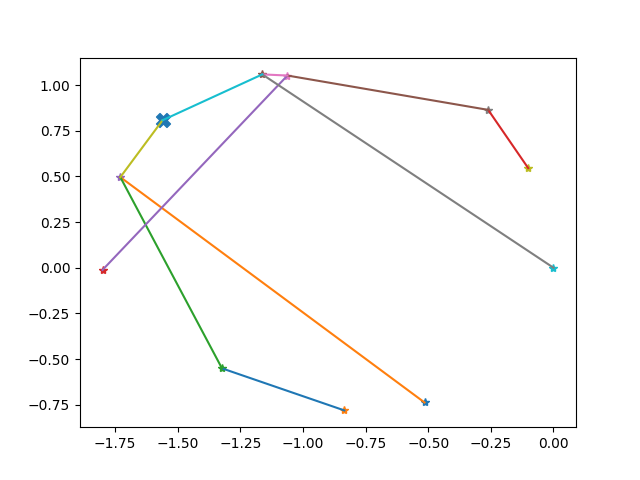
\includegraphics[scale=0.4]{opt_non_plan}
  \caption{Exemple de réveil}
  \label{fig:opt_non_plan}
\end{figure}

Dans le cas général, où les robots endormis sont disposés n'importe comment, le problème est NP-dur. Le meilleur algorithme existant, traçant le chemin des robots pour résoudre le cas général consiste en une programmation dynamique avec une complexité de $\frac{3^n}{\sqrt{n}}$ où $n$ est le nombre de robots.

Il reste cependant beaucoup de choses à explorer sur ce problème lorsque l'on considère des sous catégories du problème. Dans ce rapport, nous discuterons principalement de la pire configuration possible pour $n$ robots endormis soit la configuration qui crée le temps de réveil le plus grand. Le temps de réveil en question est appelé $\alpha_n$. On démontrera en particulier que $\alpha_5 < 3.603564775 < \alpha_4$ et on cassera des conjectures.
\clem{Il fadra qu'on revoit l'introduction, mais cela peut attendre le reste}
\subsection{Formalisation}

\subsubsection{problème du réveil des robots}

Le problème se place sur un plan muni de la distance euclidienne. Le robot réveillé est en $(0,0)$ et le problème se constitue donc de $n$ points chacun représentant les robots endormis dans le disque de rayon 1 et de centre $(0,0)$. On représente une solution au problème du réveil des robots par un arbre binaire couvrant tous les sommets. En effet, en chaque sommet, un robot entre, et on a alors 2 robots à déplacer si no le souhaite, formant alors un arbre binaire dont la racine est le premier robot éveillé.

On pondère les arêtes de notre arbre par la distance de l'arête et on considère la profondeur de l'arbre comme étant la somme des poids des arêtes depuis la racine. Dès lors, le temps de réveil d'un arbre donné est la longueur de la plus grande branche et le temps de réveil du problème est $\min_{T} \tr(T, x_1, \dots, x_n)$ où $\tr$ est le temps de réveil sachant un arbre T et l'objectif d'un algorithme est d'obtenir un arbre minimum.

On peut alors définir $\alpha_n = \max_{x_1, .., x_n} \min_T \tr(T, x_1, ..,
x_n)$

On a déjà $\alpha_1 = 1$,$\alpha_2 = \alpha_3 = 3$ et $\alpha_4 = 1 + 2\sqrt{2}$. De plus, grâce à des cônes, nous avons que $\alpha_n \leq 3 + \frac{8\pi}{\sqrt{n}}$ il est possible de faire mieux en pratique mais le résultat possède une constante plus compliquée que $8\pi$

\begin{theorem}
  Réveiller tous les robots dans un cône d'angle $\theta$ et de rayon $r$
  peut être fait en un temps $\leq r(1 + chord(theta))$
\end{theorem}


\todo[inline]{Je pense qu'il faut écrire de manière un peu plus formel, dans un
  style un peu plus académique. Par exemple :}

Dans ce rapport, nous nous travaillerons sur le plan muni de la distance
euclidienne (voir \cite{} pour d'autres métriques). Le robot réveillé débute en
$(0,0)$ et une instance du problème consiste en $n$ points représentant chacun
un robot endormi. Quitte a renormaliser, on supposera que les robots sont
disposés dans le disque de rayon 1 et de centre $(0,0)$. On représente une
solution au problème du réveil des robots par un arbre binaire couvrant tous les
sommets, enraciné en $(0, 0)$. En effet, en chaque sommet un robot entre et
réveille un autre robot: on dispose alors de deux robots à déplacer si on le
souhaite, formant ainsi un arbre binaire dont la racine est le premier robot
éveillé.

En pondérant les arêtes de notre arbre par la longueur de l'arête, on définit la
profondeur de l'arbre comme étant le maximum de la somme des poids des arêtes
depuis la racine jusqu'à une des feuilles de l'arbre. Le temps de réveil d'un
arbre $T$ est exactement la profondeur de celui-ci, on le notera
$\tr(T)$. L'objectif étant de réveiller les robots le plus rapidement possible,
le temps de réveil optimal est définit comme
$$\min_{\substack{T \text{ arbre binaire couvrant}\\ \text{enraciné en $(0,0)$}}} \tr(T, x_1, \dots,
  x_n).$$

À nombre de robots $n$ fixé, le ``pire'' cas est donc
  $$\alpha_n := \max_{x_1, \dots, x_n \in \mathbb{R}^2} \min_T \tr(T, x_1, \dots,
x_n)$$

Il est assez facile de prouver que  $\alpha_1 = 1$ et $\alpha_2 = \alpha_3 = 3$.
Pour $n=4$, on peut prouver (\cite{}) que $\alpha_4 = 1 + 2\sqrt{2}$.
Gavoille, (lister les autres) ont prouvé dans \cite{} que $\alpha_n \leq 3 +
\frac{8\pi}{\sqrt{n}}$. Il est possible de faire mieux en pratique mais la borne
ferait intervenir une constante plus compliquée que $8\pi$.

Dans la suite, nous utiliserons régulièrement le résultat suivant dû à Gavoille
( et...) :
\begin{theorem}[\cite{}]
  Il faut au plus $r(1 + \chord(\theta))$ pour réveiller tous les robots dans un
  cône de rayon $r$ et d'angle $\theta$, à partir d'un robot éveillé
  initialement placé au centre du cône.
\end{theorem}